% Options for packages loaded elsewhere
\PassOptionsToPackage{unicode}{hyperref}
\PassOptionsToPackage{hyphens}{url}
%
\documentclass[
]{article}
\usepackage{lmodern}
\usepackage{amssymb,amsmath}
\usepackage{ifxetex,ifluatex}
\ifnum 0\ifxetex 1\fi\ifluatex 1\fi=0 % if pdftex
  \usepackage[T1]{fontenc}
  \usepackage[utf8]{inputenc}
  \usepackage{textcomp} % provide euro and other symbols
\else % if luatex or xetex
  \usepackage{unicode-math}
  \defaultfontfeatures{Scale=MatchLowercase}
  \defaultfontfeatures[\rmfamily]{Ligatures=TeX,Scale=1}
\fi
% Use upquote if available, for straight quotes in verbatim environments
\IfFileExists{upquote.sty}{\usepackage{upquote}}{}
\IfFileExists{microtype.sty}{% use microtype if available
  \usepackage[]{microtype}
  \UseMicrotypeSet[protrusion]{basicmath} % disable protrusion for tt fonts
}{}
\makeatletter
\@ifundefined{KOMAClassName}{% if non-KOMA class
  \IfFileExists{parskip.sty}{%
    \usepackage{parskip}
  }{% else
    \setlength{\parindent}{0pt}
    \setlength{\parskip}{6pt plus 2pt minus 1pt}}
}{% if KOMA class
  \KOMAoptions{parskip=half}}
\makeatother
\usepackage{xcolor}
\IfFileExists{xurl.sty}{\usepackage{xurl}}{} % add URL line breaks if available
\IfFileExists{bookmark.sty}{\usepackage{bookmark}}{\usepackage{hyperref}}
\hypersetup{
  pdftitle={TP1 Econometría Avanzada},
  pdfauthor={Casiano, Denys; Daboin, Carlos y Quispe, Anzony},
  hidelinks,
  pdfcreator={LaTeX via pandoc}}
\urlstyle{same} % disable monospaced font for URLs
\usepackage[left=2.5cm,right=2.5cm,top=1.5cm,bottom=2cm]{geometry}
\usepackage{graphicx,grffile}
\makeatletter
\def\maxwidth{\ifdim\Gin@nat@width>\linewidth\linewidth\else\Gin@nat@width\fi}
\def\maxheight{\ifdim\Gin@nat@height>\textheight\textheight\else\Gin@nat@height\fi}
\makeatother
% Scale images if necessary, so that they will not overflow the page
% margins by default, and it is still possible to overwrite the defaults
% using explicit options in \includegraphics[width, height, ...]{}
\setkeys{Gin}{width=\maxwidth,height=\maxheight,keepaspectratio}
% Set default figure placement to htbp
\makeatletter
\def\fps@figure{htbp}
\makeatother
\setlength{\emergencystretch}{3em} % prevent overfull lines
\providecommand{\tightlist}{%
  \setlength{\itemsep}{0pt}\setlength{\parskip}{0pt}}
\setcounter{secnumdepth}{-\maxdimen} % remove section numbering
\usepackage{booktabs} \usepackage{longtable} \usepackage{array} \usepackage{multirow} \usepackage{wrapfig} \usepackage{float} \floatplacement{figure}{H}

\title{TP1 Econometría Avanzada}
\author{Casiano, Denys; Daboin, Carlos y Quispe, Anzony}
\date{2022-04-09}

\begin{document}
\maketitle

\hypertarget{discusion-del-estimador-between}{%
\subsection{1. Discusion del estimador
between}\label{discusion-del-estimador-between}}

\emph{Discuta el modelo estimado (comente acerca de la validez del
estimador between y potenciales sesgos) y comente los resultados
obtenidos, en particular para las variables de justicia criminal.}

\hypertarget{posibles-problemas-de-heterogeneidad-no-observable}{%
\subsection{2. Posibles problemas de heterogeneidad no
observable}\label{posibles-problemas-de-heterogeneidad-no-observable}}

\emph{Explique por qué es muy posible que la presencia de heterogeneidad
no observable a nivel de condado haga que las estimaciones anteriores
sean sesgadas. } Dos condados pueden ser diferentes en caracteristicas
que no-observables y que son \emph{confounders} (correlacionadas con la
tasa de criminalidad y las variables explicativas.)

Por ejemplo, es plausible que haya distintos niveles de subreporte del
crimen entre distintos condados. De ser esto cierto, un condado similar
a los demas donde se reporte una menor proporcion de los crimines tendra
una menor tasa de criminalidad (variable dependiente) y mayores tasas de
arresto, lo que sesgaria negativamente el efecto de las tasas de arresto
sobre la criminalidad, haciendolo parecer de mayor magnitud.

\emph{Realice una estimación con efectos fijos por condado.}

\emph{Discuta por qué esta alternativa resolvería el problema de sesgo.
}\\
Un estimador de efectos fijos estaria exento de toda la variabilidad
atribuible a los condados, por lo que se esta controlando por todos los
no-observables que varian en este nivel.

Acerca del ejemplo anterior, un estimador de efectos fijos (tambien
llamado \emph{within}) nos permitiria hubiese corregido las bajas tasas
de criminalidad y las altas tasas de arresto de nuestro condado con alto
subreporte, haciendolo comparable a los demas.

\emph{Testee formalmente la hipótesis nula de ausencia de efectos fijos.
}

\emph{A la luz del trabajo de CyT, discuta las principales diferencias
encontradas con las estimaciones anteriores.}

\hypertarget{including-plots}{%
\subsection{Including Plots}\label{including-plots}}

You can also embed plots, for example:

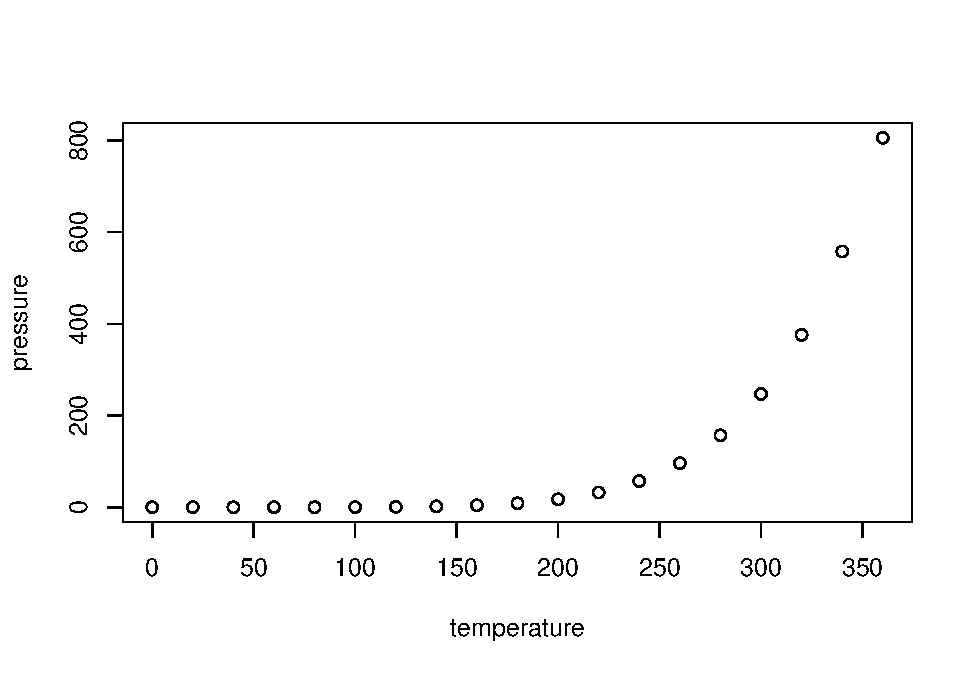
\includegraphics{TP2_Econometria_Avanzada_Casiano_Daboin_Quispe_files/figure-latex/pressure-1.pdf}

Note that the \texttt{echo\ =\ FALSE} parameter was added to the code
chunk to prevent printing of the R code that generated the plot.

\end{document}
